\documentclass{article}

\usepackage[final]{neurips_2023}

\usepackage[utf8]{inputenc} % allow utf-8 input
\usepackage[T1]{fontenc}    % use 8-bit T1 fonts
\usepackage{hyperref}       % hyperlinks
\usepackage{url}            % simple URL typesetting
\usepackage{booktabs}       % professional-quality tables
\usepackage{amsfonts}       % blackboard math symbols
\usepackage{nicefrac}       % compact symbols for 1/2, etc.
\usepackage{microtype}      % microtypography
\usepackage{xcolor}         % colors
\usepackage{natbib}         % bibliography
\usepackage{graphicx}       % for figures

\title{Program of Thoughts Prompting for Accurate Numerical Reasoning}



% The \author macro works with any number of authors. There are two commands
% used to separate the names and addresses of multiple authors: \And and \AND.
%
% Using \And between authors leaves it to LaTeX to determine where to break the
% lines. Using \AND forces a line break at that point. So, if LaTeX puts 3 of 4
% authors names on the first line, and the last on the second line, try using
% \AND instead of \And before the third author name.


\author{%
SoonHo Kim \\
Team 14 - 20200703 \\
}


\begin{document}


\maketitle


\section{Problem Definition}

Numerical reasoning has been a long-standing challenge in natural language processing (NLP). Existing methods like Chain-of-Thought (CoT) prompting enable large language models (LLMs) to perform step-by-step reasoning for math word problems. However, CoT has a fundamental limitation in that LLMs must handle both reasoning and computation within natural language, which often leads to incorrect results due to arithmetic errors, especially with large numbers or iterative processes. The paper proposes a solution that separates these two responsibilities.

\section{Proposed Method}

\begin{figure}[h]
  \centering
  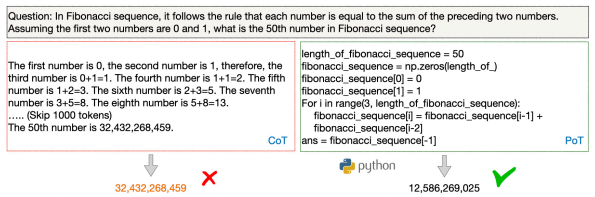
\includegraphics[width=0.8\linewidth]{figure1.png}
  \caption{Comparison between Chain of Thoughts and Program of Thoughts~\cite{chen2022program}.}
  \label{fig:cot-vs-pot}
\end{figure}

The paper introduces a new method called \textbf{Program of Thoughts (PoT)} prompting. Instead of solving math problems entirely through language, PoT allows LLMs to express the reasoning process using code (e.g., Python), and offloads actual computation to a program interpreter. This separation enables models to focus on logical structure while leveraging the precision and speed of traditional computing systems. PoT also uses semantically meaningful variable names and multi-step decomposition, which significantly improves performance across several math and finance benchmarks. Compared to CoT, PoT achieves an average 12\% improvement across datasets like GSM8K, AQuA, and FinQA.

\section{Discussion}

Our team’s project focuses on building a general game-playing AI using LLMs, with chess as the primary testbed. In chess, a game state leads to many deterministic possibilities that are best handled through algorithmic simulation. Inspired by PoT, we plan to offload these deterministic calculations (e.g., generating legal moves, evaluating material scores) to a Python-based backend. The LLM will then focus only on strategic reasoning, such as choosing the best move based on the situation. This division allows for more accurate move predictions and better interpretability, much like how PoT achieves more robust reasoning by separating logic and calculation.



\newpage
\bibliographystyle{plain}
\bibliography{reference}

\end{document}